\documentclass[a4paper, 12pt]{article}
\usepackage[utf8]{inputenc}
\usepackage[english, ukrainian]{babel}

\usepackage{amsmath, amssymb}
\usepackage{multicol}
\usepackage{graphicx}
\usepackage{float}

\allowdisplaybreaks
\setlength\parindent{0pt}
\numberwithin{equation}{subsection}

\usepackage{hyperref}
\hypersetup{unicode=true,colorlinks=true,linktoc=all,linkcolor=red}

\numberwithin{equation}{subsection}

\renewcommand{\bf}[1]{\textbf{#1}}
\renewcommand{\it}[1]{\textit{#1}}
\newcommand{\bb}[1]{\mathbb{#1}}
\renewcommand{\cal}[1]{\mathcal{#1}}

\renewcommand{\epsilon}{\varepsilon}
\renewcommand{\phi}{\varphi}

\DeclareMathOperator{\diam}{diam}
\DeclareMathOperator{\rang}{rang}
\DeclareMathOperator{\const}{const}

\newenvironment{system}{%
  \begin{equation}%
    \left\{%
      \begin{aligned}%
}{%
      \end{aligned}%
    \right.%
  \end{equation}%
}
\newenvironment{system*}{%
  \begin{equation*}%
    \left\{%
      \begin{aligned}%
}{%
      \end{aligned}%
    \right.%
  \end{equation*}%
}

\makeatletter
\newcommand*{\relrelbarsep}{.386ex}
\newcommand*{\relrelbar}{%
  \mathrel{%
    \mathpalette\@relrelbar\relrelbarsep%
  }%
}
\newcommand*{\@relrelbar}[2]{%
  \raise#2\hbox to 0pt{$\m@th#1\relbar$\hss}%
  \lower#2\hbox{$\m@th#1\relbar$}%
}
\providecommand*{\rightrightarrowsfill@}{%
  \arrowfill@\relrelbar\relrelbar\rightrightarrows%
}
\providecommand*{\leftleftarrowsfill@}{%
  \arrowfill@\leftleftarrows\relrelbar\relrelbar%
}
\providecommand*{\xrightrightarrows}[2][]{%
  \ext@arrow 0359\rightrightarrowsfill@{#1}{#2}%
}
\providecommand*{\xleftleftarrows}[2][]{%
  \ext@arrow 3095\leftleftarrowsfill@{#1}{#2}%
}
\makeatother

\newcommand{\NN}{\mathbb{N}}
\newcommand{\ZZ}{\mathbb{Z}}
\newcommand{\QQ}{\mathbb{Q}}
\newcommand{\RR}{\mathbb{R}}
\newcommand{\CC}{\mathbb{C}}

\newcommand{\Max}{\displaystyle\max\limits}
\newcommand{\Sup}{\displaystyle\sup\limits}
\newcommand{\Sum}{\displaystyle\sum\limits}
\newcommand{\Int}{\displaystyle\int\limits}
\newcommand{\Iint}{\displaystyle\iint\limits}
\newcommand{\Lim}{\displaystyle\lim\limits}

\newcommand*\diff{\mathop{}\!\mathrm{d}}

\newcommand*\rfrac[2]{{}^{#1}\!/_{\!#2}}


\title{{\Huge МАТЕМАТИЧНА ФІЗИКА}}
\author{Скибицький Нікіта}
\date{\today}

\usepackage{amsthm}
\usepackage[dvipsnames]{xcolor}
\usepackage{thmtools}
\usepackage[framemethod=TikZ]{mdframed}

\theoremstyle{definition}
\mdfdefinestyle{mdbluebox}{%
	roundcorner = 10pt,
	linewidth=1pt,
	skipabove=12pt,
	innerbottommargin=9pt,
	skipbelow=2pt,
	nobreak=true,
	linecolor=blue,
	backgroundcolor=TealBlue!5,
}
\declaretheoremstyle[
	headfont=\sffamily\bfseries\color{MidnightBlue},
	mdframed={style=mdbluebox},
	headpunct={\\[3pt]},
	postheadspace={0pt}
]{thmbluebox}

\mdfdefinestyle{mdredbox}{%
	linewidth=0.5pt,
	skipabove=12pt,
	frametitleaboveskip=5pt,
	frametitlebelowskip=0pt,
	skipbelow=2pt,
	frametitlefont=\bfseries,
	innertopmargin=4pt,
	innerbottommargin=8pt,
	nobreak=true,
	linecolor=RawSienna,
	backgroundcolor=Salmon!5,
}
\declaretheoremstyle[
	headfont=\bfseries\color{RawSienna},
	mdframed={style=mdredbox},
	headpunct={\\[3pt]},
	postheadspace={0pt},
]{thmredbox}

\declaretheorem[style=thmbluebox,name=Теорема,numberwithin=subsubsection]{theorem}
\declaretheorem[style=thmbluebox,name=Лема,numberwithin=subsubsection]{lemma}
\declaretheorem[style=thmbluebox,name=Твердження,numberwithin=subsubsection]{proposition}
\declaretheorem[style=thmbluebox,name=Принцип,numberwithin=subsubsection]{th_principle}
\declaretheorem[style=thmbluebox,name=Закон,numberwithin=subsubsection]{law}
\declaretheorem[style=thmbluebox,name=Закон,numbered=no]{law*}
\declaretheorem[style=thmbluebox,name=Формула,numberwithin=subsubsection]{th_formula}
\declaretheorem[style=thmbluebox,name=Рівняння,numberwithin=subsubsection]{th_equation}
\declaretheorem[style=thmbluebox,name=Умова,numberwithin=subsubsection]{th_condition}
\declaretheorem[style=thmbluebox,name=Наслідок,numberwithin=subsubsection]{corollary}

\declaretheorem[style=thmredbox,name=Приклад,numberwithin=subsubsection]{example}
\declaretheorem[style=thmredbox,name=Приклади,sibling=example]{examples}

\declaretheorem[style=thmredbox,name=Властивість,numberwithin=subsubsection]{property}
\declaretheorem[style=thmredbox,name=Властивості,sibling=property]{properties}

\mdfdefinestyle{mdgreenbox}{%
	skipabove=8pt,
	linewidth=2pt,
	rightline=false,
	leftline=true,
	topline=false,
	bottomline=false,
	linecolor=ForestGreen,
	backgroundcolor=ForestGreen!5,
}
\declaretheoremstyle[
	headfont=\bfseries\sffamily\color{ForestGreen!70!black},
	bodyfont=\normalfont,
	spaceabove=2pt,
	spacebelow=1pt,
	mdframed={style=mdgreenbox},
	headpunct={ --- },
]{thmgreenbox}

\mdfdefinestyle{mdblackbox}{%
	skipabove=8pt,
	linewidth=3pt,
	rightline=false,
	leftline=true,
	topline=false,
	bottomline=false,
	linecolor=black,
	backgroundcolor=RedViolet!5!gray!5,
}
\declaretheoremstyle[
	headfont=\bfseries,
	bodyfont=\normalfont\small,
	spaceabove=0pt,
	spacebelow=0pt,
	mdframed={style=mdblackbox}
]{thmblackbox}

\declaretheorem[name=Вправа,numberwithin=subsubsection,style=thmblackbox]{exercise}
\declaretheorem[name=Зауваження,numberwithin=subsubsection,style=thmgreenbox]{remark}
\declaretheorem[name=Визначення,numberwithin=subsubsection,style=thmblackbox]{definition}

\newtheorem{problem}{Задача}[subsection]
\newtheorem{sproblem}[problem]{Задача}
\newtheorem{dproblem}[problem]{Задача}
\renewcommand{\thesproblem}{\theproblem$^{\star}$}
\renewcommand{\thedproblem}{\theproblem$^{\dagger}$}
\newcommand{\listhack}{$\empty$\vspace{-2em}} 

\theoremstyle{remark}
\newtheorem*{solution}{Розв'язок}


\begin{document}

\tableofcontents

\setcounter{section}{3}
\setcounter{subsection}{3}
\setcounter{subsubsection}{13}
\setcounter{theorem}{19}
\setcounter{equation}{107}

\subsection{Моделі руху в'язкої рідини}

\begin{definition}[в'язкості рідини]
	\it{В'язкість рідини} --- це властивість чинити опір пересуванню її часток, яка характеризує ступінь її плинності та рухливості.
\end{definition}

Як видно з визначення, в'язкість є властивістю рідини, що рухається, і в стані спокою не виявляється. Наявність сил внутрішнього тертя рідини, що рухається, уперше встановив Ньютон, згодом російський вчений В. Н. Петров у 1888 р. привів математичний вираз для сили тертя. \medskip

Нехай шар рідини $A$ рухається зі швидкістю $v$, а шар рідини $B$ зі швидкістю $v + \diff v$, відстань між шарами $\diff y$:
\begin{figure}[H]
	\centering
	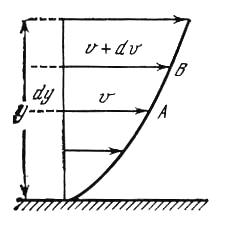
\includegraphics[]{img/12-1.png}
\end{figure}

У введених позначеннях сила тертя $T$ між двома шарами рідини задається формулою
\begin{equation}
	T = - \mu F\frac{\diff v}{\diff y},
\end{equation}
де $\mu$ --- динамічний коефіцієнт в'язкості, $F$ --- площа стикання двох шарів рідини. Знак мінус вказує на те , що тертя діє в напряму протилежному рухові. \medskip

Закони, що описують процеси руху в'язкої рідини, залишаються тими що і для ідеальної рідини, але при цьому з'являється додатковий механізм передачі імпульсу та енергії. \medskip

\begin{law}[збереження маси у вигляді рівняння нерозривності]
	Залишається незмінним:
	\begin{equation}
		\frac{\partial \rho}{\partial t} + \nabla \cdot \Big(\rho \vecf V\Big) = 0.		
	\end{equation}
\end{law}

\subsubsection{Закон збереження імпульсу}

Нагадаємо вигляд потоку імпульсу для ідеальної рідини, що проходить через елементарну поверхню $\diff S$ в одиницю часу:
\begin{equation}
	\diff \vecf I = \Big(\rho V_n \vecf V + p \vec n \Big) \diff S.
\end{equation}

\begin{remark}
	Нагадаємо, що $V_n$ --- нормальна складова векторного поля $\vecf V$, тобто
	\begin{equation}
		V_n = \Big\langle \vecf V, \vec n \Big\rangle.
	\end{equation}
\end{remark}

Дамо
\begin{definition}[щільності потоку імпульсу]
	Введемо тензорну величину \it{щільності потоку імпульсу}:
	\begin{equation}
		\bm{\Pi} = \rho 
		\begin{pmatrix}
			V_1 V_1 & V_1 V_2 & V_1 V_3 \\
			V_2 V_1 & V_2 V_2 & V_2 V_3 \\
			V_3 V_1 & V_3 V_2 & V_3 V_3
		\end{pmatrix}
		+
		\begin{pmatrix}
			1 & 0 & 0 \\
			0 & 1 & 0 \\
			0 & 0 & 1
		\end{pmatrix}
		p.
	\end{equation}
\end{definition}

Тоді закон збереження маси у вигляді рівняння нерозривності можна записати у вигляді: 
\begin{equation}
	\diff \vecf I = \Big\langle \bm{\Pi}, \vec n \Big\rangle \diff S.
\end{equation}

\begin{law}[збереження імпульсу ідеальної рідини]
	З використанням тензору щільності потоку імпульсу $\bm{\Pi}$ матиме вигляд:
	\begin{equation}
		\frac{\partial \rho \vecf V}{\partial t} + \nabla \cdot \bm{\Pi} = 0.
	\end{equation}
\end{law}

Для в'язкої рідини, у випадку тривимірних рухів додатковий механізм переносу потоку імпульсу має тензорну природу і задається через симетричний тензор в'язких напружень.

\begin{definition}[симетричного тензору в'язких напружень]
	\it{Симетричним тензором в'язких напружень} називається тензор, компоненти якого визначаються наступними рівняннями: 
	\begin{equation}
		\sigma_{ik} = \eta \left( \frac{\partial V_i}{\partial x_k} + \frac{\partial V_k}{\partial x_i} - \frac{2}{3} \delta_{ik} \Sum_{l = 1}^3 \frac{\partial V_l}{\partial x_l}\right) + \xi \delta_{ik} \Sum_{l = 1}^3 \frac{\partial V_l}{\partial x_l},
	\end{equation}
	де $\xi, \eta > 0$ --- коефіцієнти першої та другої в'язкості, $\delta_{ik}$ --- символ Кронекера, а
	\begin{equation}
		\Sum_{l = 1}^3 \frac{\partial V_l}{\partial x_l} = \nabla \cdot \vecf V.
	\end{equation}
\end{definition}

\begin{remark}
	Рідина \it{ідеальна}, коли $\xi = \eta = 0$.
\end{remark}

Таким чином для в'язкої рідини симетричний тензор щільності потоку імпульсу приймає вигляд:
\begin{equation}
	\bm{\Pi}_{ik} = \rho V_i V_k + p \delta_{ik} - \sigma_{ik}.
\end{equation}

Використовуючи загальний вигляд тензору потоку імпульсу для в'язкої рідини, маємо
\begin{law}[збереження імпульсу]
	Також можна записати у розгорнутому вигляді:
	\begin{equation}
		\frac{\partial \rho \vecf V}{\partial t} + \nabla \cdot \Big(\rho \vecf V \vecf V^\intercal\Big) + \nabla p = \eta \Delta \vecf V + \left( \xi + \frac{\eta}{3} \right) \nabla \Big(\nabla \cdot \vecf V \Big).
	\end{equation}
\end{law}

\begin{remark}
	Як видно, тут ми вважаємо, що $\vecf V$ --- вектор-стовпчик. У випадку вектора-рядка потрібно було б записати $\vecf V^\intercal \vecf V$ замість $\vecf V \vecf V^\intercal$.
\end{remark}

\begin{remark}
	Закон збереження імпульсу для в'язкої рідини у випадку нестисливої рідини, тобто коли $\rho \equiv \const$ має простіший вигляд.
\end{remark}
	
Рівняння нерозривності приймає вигляд $\nabla \cdot \vecf V = 0$. \medskip

Отже, поле швидкості є соленоїдальним, тобто
\begin{equation}
	\frac{\partial \rho \vecf V}{\partial t} + \nabla \cdot \Big(\rho \vecf V \vecf V^\intercal\Big) = - \nabla p + \eta \Delta \vecf V,
\end{equation}
або
\begin{equation}
	\frac{\partial \vecf V}{\partial t} + \nabla \cdot \Big(\vecf V \vecf V^\intercal\Big) = - \frac{\nabla p}{\rho} + \frac{\eta}{\rho} \Delta \vecf V.
\end{equation}

\subsubsection{Закон збереження енергії}

Запишемо потік енергії для ідеальної рідини:
\begin{equation}
	\diff \vecf E = \left( \rho \vecf V \frac{|\vecf V|^2}{2} + \rho \epsilon \vecf V + p \vecf V\right) \vec n \diff S,
\end{equation}
або
\begin{equation}
	\diff \vecf E = \rho V_n \left( \frac{|\vecf V|^2}{2} + \epsilon + \frac{p}{\rho}\right)\diff S.
\end{equation}

Замість скалярної величини тиску $p$ для ідеальної рідини введемо тензор напружень для в'язкої рідини $\dot{\bf{P}}_{ik} = p \delta_{ik} - \sigma_{ik}$. \medskip

Тоді матимемо 
\begin{equation}
	\diff \vecf E = \rho \left\langle\left(\left( \frac{|\vecf V|^2}{2} + \epsilon \right) I + \frac{\dot{\bf{P}}}{\rho} \right)\vecf V, \vec n \right\rangle,
\end{equation}
де $I$ --- одинична матриця. \medskip

Можна записати
\begin{law}[інтегральний закон збереження повної енергії]
	\begin{multline}
		\Iiint_G \rho \left. \left( \frac{|\vecf V|^2}{2} + \epsilon\right)^2 \right|_{t_1}^{t_2} \diff G + \\
		+\Int_{t_1}^{t_2} \Iint_S \left\langle \left(\rho \left(\frac{|\vecf V|^2}{2} + \epsilon \right)I+\frac{\dot{\bf{P}}}{\rho}\right),\vec n\right\rangle \diff S \diff t = 0.
	\end{multline}
\end{law}

Звідси, 
\begin{law}[збереження повної енергії для в'язкої рідини]
	\begin{equation}
		\frac{\partial}{\partial t} \left( \rho \left( \frac{|\vecf V|^2}{2} + \epsilon\right)\right) + \nabla \cdot \left( \left( \rho \left(\frac{|\vecf V|^2}{2} + \epsilon\right)I + \dot{\bf{P}}\right) \vecf V \right) = 0.
	\end{equation}
\end{law}

Якщо рідина не тільки в'язка, а й теплопровідна, то з'являється ще один механізм передачі енергії --- теплопровідність, тоді другий доданок матиме вигляд:
\begin{equation}
	\nabla \cdot \left( \left( \rho \left(\frac{|\vecf V|^2}{2} + \epsilon\right)I + \dot{\bf{P}}\right) \vecf V + \vecf Q\right)
\end{equation}

де $\vecf Q$ --- потік тепла,
\begin{equation}
	\vecf Q = - k \nabla \epsilon,
\end{equation}
а $k$ --- коефіцієнт теплопровідності. \medskip

Отже, отримали
\begin{th_equation}[які описують рух в'язкої рідини]
	Ця система складається з рівняння нерозривності (закону збереження маси), закону збереження імпульсу, і закону збереження повної енергії, та замикається рівнянням стану
	\begin{equation}
		\epsilon = \epsilon(p, \rho).
	\end{equation}
\end{th_equation}

\begin{remark}
	При переході від моделі ідеальної до моделі в'язкої рідини збільшується порядок рівнянь з першого на другий.
\end{remark}

\subsubsection{Додаткові умови}

Початкові умови:  				(4.16).
В початковий момент часу задаються усі невідомі параметри.
Граничні умови на поверхні тіла 
Якщо нерухоме тіло обтікається в'язкою рідиною, то за рахунок молекулярних сил, в'язка рідина прилипає до поверхні тіла, тобто виконується умова: 	  									(4.17). 
Якщо поверхня тіла рухається зі швидкістю   та на його поверхні для в'язкої рідини виконується умова 
 									(4.17/).
Умови (4.17), (4.17/) називаються умовами приліпання.

\subsubsection{Умови на поверхні розділу двох середовищ}

У випадку, коли два середовища розділені рухомою поверхнею, (дві рідини, що не змішуються) то на межі розділу двох середовищ, мають бути задані дві умови: 
динамічна:   							(4.18),
статична:   або	 	 		(4.19)
Співвідношення (4.18) вказує на те, що вектор швидкості на поверхні розділу двох середовищ є неперервним, а сама поверхня рухається з місцевою швидкістю середовища  . Співвідношення (4.19) вказує на те, що рівнодіюча сил на поверхні розділу середовищ дорівнює нулю,   - вектори зовнішньої нормалі,  

\subsubsection{Граничні умови на вільній поверхні}

Вільною поверхнею будемо називати поверхню утворену частинками в'язкої рідини на яку діє деяка зовнішня сила. Нехай   - рівняння вільної поверхні, де  - невідома функція, тоді співвідношення 
 									 (4.20) виражає умову непротікання рідини через поверхню (через вільну поверхню рідина не перетікає), а також вказує на те, що сама вільна поверхня переміщується з місцевою швидкістю руху рідини.
На вільну поверхню також діє зовнішня сила, яка задається тензорним співвідношенням:  							(4.21).
Скалярна форма (4.21) має вигляд: 
 						(4.21/),    де   – компоненти вектора зовнішніх сил, що діють на поверхні  ;

\subsection{Математичні моделі електростатики}

З курсу фізики відомо, що при певних умовах окремі тіла (діелектрики) можуть отримувати додаткові електричні заряди (відбувається електризація). Наявність електричних зарядів проявляється у взаємодії заряджених тіл між собою (тіла притягуються або відштовхуються). \medskip

Відомо, що існують два види електричних зарядів, які умовно поділяються на додатні та від'ємні. Будь-який електричний заряд утворюється як сукупність елементарних неподільних за величиною зарядів. Носієм такого елементарного від'ємного заряду є електрон, носієм елементарного позитивного заряду може бути протон. Величину елементарного заряду традиційно позначають $\mathrm{e}$. \medskip

Будь-який електричний заряд утворюється як сукупність елементарних зарядів $q = \pm N \mathrm{e}$. \medskip

Якщо заряджені частинки в тілі можуть більш менш вільно пересуватися в межах тіла, то кажуть, що тіло здатне проводити електричний струм. Носіями зарядів можуть бути не тільки електрони, але іони (атоми, що приєднали до себе або згубили один чи декілька електронів). \medskip

Будемо розглядати точкові заряди. Тобто заряджені тіла, геометричними розмірами яких можна нехтувати, вважаючи їх точкою. Взаємодія точкових електричних зарядів полягає в виникненні сили тяжіння або відштовхування. Величина цієї сили експериментально встановлена Кулоном у вигляді фізичного закону
\begin{law}[Кулона]
	Виконується співвідношення
	\begin{equation}
		f = k \frac{q_1 q_2}{|r|^2},
	\end{equation}
	де  $k$ --- коефіцієнт пропорційності, який залежить від середовища в якому відбувається взаємодії, $q_1$, $q_2$ --- величини зарядів, $r$ --- відстань між зарядами.
\end{law}

Враховуючи векторний характер сили, закон Кулона можна записати в векторному вигляді
\begin{equation}
	\vec f = k \frac{q_1 q_2}{|r|^3} \vec r
\end{equation}

Якщо характеризувати силу, з якою заряд $q_1$ діє на заряд $q_2$, то радіус вектор $\vec r$ направлений від $q_1$ до $q_2$. При цьому сила з якою заряд $q_2$ діє на заряд $q_1$ рівна за величиною та протилежна за напрямом. Закон Кулона в вакуумі має вигляд:
\begin{equation}
	\vec f = \frac{1}{4 \pi \epsilon_0} \frac{q_1q_2}{|r|^3} \vec r,
\end{equation}
дк $\epsilon_0$ називають електричною постійною.

\subsubsection{Електричне поле. Напруженість електричного поля}

Взаємодія між електричними зарядами відбувається через електричне поле. Будь-який заряд змінює властивості оточуючого середовища створюючи в ньому електричне поле. Це поле проявляє себе у тому, що розташований в цьому полі заряд буде знаходитись під дією сили. \medskip

Для дослідження поля використовують пробний заряд, який обирають невеликим за величиною і розмірами (точковий заряд). Згідно до закону Кулона сила $\vec f$, що діє на пробний заряд   полем точкового заряду величини $q'$ записується у вигляді
\begin{equation}
	\vec f = q' \left( \frac{1}{4 \pi \epsilon_0} \frac{q}{|r|^3} \vec r \right)
\end{equation}

З цієї формули видно, що сила $\vec f$ залежить від $q'$.

\begin{definition}[напруженості електричного поля]
	Характеристикою електричного поля, яка не залежить від величини пробного заряду є
	\begin{equation}
		E = \frac{\vec f}{q},
	\end{equation}
	яку називають \it{напруженістю електричного поля}.
\end{definition}

\begin{remark}
	Її також можна визначити як силу, що діє на одиничний пробний заряд.
\end{remark}

Таким чином, з напруженість електричного поля точкового заряду $q$ визначається за формулою:
\begin{equation}
	\vecf E = \frac{1}{4 \pi \epsilon_0} \frac{q}{|r|^3} \vec r,
\end{equation}
де вектор $\vec r$ направлений від точки розташування заряду $q$ до точки знаходження пробного заряду. 

\subsubsection{Суперпозиція полів}

Дослідним шляхом встановлено, що у випадку, коли поле утворюється декількома точковими зарядами, то сумарна сила, яка діє на пробний заряд дорівнює векторній сумі від дії кожної окремої сили, тобто  
 									(5.6).
Остання формула носить назву принципу суперпозиції електричних полів.
Нехай в точках   простору розташовані заряди величиною    , тоді згідно до принципу суперпозиції електричних полів, можна записати:
 								(5.7),
де   = ,   - довжина цього вектора. 
У випадку, коли в області   трьохвимірного простору заряди розташовані щільно і щільність їх розташування задана деякою функцією  , то напруженість електричного поля визначається у вигляді інтегралу:
  							(5.7').

\subsubsection{Потік векторного поля. Теорема Гауса}

Потоком векторного поля   через поверхню   будемо називати величину 
 									(5.8).
Розглянемо замкнену поверхню   всередині якої знаходиться точковий заряд  , тоді потік векторного поля цього заряду можна розрахувати за формулою (5.8), або враховуючи (5.7') маємо:
 								(5.9), 		де   - вектор направлений від точки розташування заряду до змінної точки поверхні  .
Неважко перевірити, що  					(5.10) 
тоді  		  			(5.10').
В наступних лекціях, при вивченні гармонічних функцій ми покажемо, що інтеграл (5.10') дорівнює  .
Таким чином потік напруженості векторного поля одного точкового заряду дорівнює величині цього заряду поділеному на електричну постійну.
Враховуючи принцип суперпозиції електричного поля можна сформулювати наступну теорему:
Теорема 1 (Гауса про значення потоку електричного поля через замкнену поверхню) Потік напруженості векторного поля через замкнену поверхню   тіла дорівнює алгебраїчній сумі зарядів, що знаходяться всередині цієї поверхні поділеній на діелектричну сталу   	
 										(5.11).
Якщо заряд розподілений всередині замкненого об'єму, обмеженого поверхнею   з об'ємною густиною   , то теорема Гауса буде мати вигляд  									(5.11').
Поряд з напруженістю векторного поля  , для опису електричного поля вводять величину  , яка називається електричним зміщенням. Для вакууму вона визначається   									(5.12).
Формула Гауса приймає вид:  	 				(5.13)

\subsubsection{Робота сил електростатичного поля. Потенціал електростатичного поля}

Відомо, що робота в силовому полі, виконана вздовж деякого контуру C силою   обчислюється у вигляді  криволінійного інтегралу другого роду за формулою 
 . Відповідно, для електричного поля ця робота може бути записана у вигляді   							(5.14), 
інтеграл (5.14) будемо називати циркуляцією векторного поля вздовж контуру  
Введемо величину  		  і назвемо її потенціалом електростатичного поля одиничного точкового заряду, розташованого в точці початку координат. Враховуючи (5.10), легко бачити, що  , тобто векторне поле одиничного точкового заряду є потенціальним. Аналогічна властивість має місце і для поля розподілених в об'ємі зарядів. 
Легко перевірити, що формула (5.7') може бути переписана у вигляді  							(5.7'').
Враховуючи потенційність векторного поля, роботу в такому полі можна обчислити 
 					(5.15), якщо  ,то  .
Зрозуміло, що  циркуляція  електростатичного поля вздовж довільного замкненого контуру дорівнює нулю тобто  				(5.15').
Виходячи з (5.15) можна визначити фізичний зміст потенціалу електростатичного поля в заданій точці. Потенціал електростатичного поля – це робота яку необхідно здійснити, щоб перемістити одиничний точковий заряд з нескінченно віддаленої точки простору у задану точку. Ця робота не залежить від шляху переміщення, а залежить лише від положення точки.
Електричне поле утворене сукупністю точкових зарядів, або розподілених у просторі з деякою щільністю також залишається потенціальним, а значить допускає існування скалярної функції  , такої, що  .		(5.16).
Враховуючі теорему Гауса та формулу Остроградського – Гауса отримаємо  рівняння  , або враховуючи (5.16) отримаємо  рівняння:
   або 	 						(5.17).
(5.17) представляє собою основне рівняння електростатики для вакууму.
Крім теореми Гауса при постановці граничних задач електростатики необхідно враховувати різні граничні режими електростатичного поля, зокрема:
Всередині провідника електричне поле   завжди дорівнює нулю, таким чином потенціал  . Ця константа має одне і теж саме значення у системі з'єднаних між собою провідними зв'язками провідників. Якщо провідники відокремлені один від одного, то   для кожного провідника має своє окреме значення.


\end{document}